\section{Related Work}
%\acrshort{tcp} have two basic problems. 1) \acrshort{tcp} is tightly coupled with \acrshort{ip}, 2) \acrshort{tcp}'s slow-start mechanism is ill-suited for short-lived connection. 
%To solve the first problem. i.e. decoupling \acrshort{tcp} and \acrshort{ip}, first approach is to solve it from network. So, we got Mobile IP, \acrfull{hip}, \acrfull{shim6}. These protocols try to hide the information that underlying path has been changed. It \acrshort{tcp}'s congestion control suffers from this.
%
%The another approach is to solve it from the transport layer. For this we got \acrfull{sctp} and \acrfull{mptcp}. \acrshort{sctp} is similar to \acrshort{tcp}, but it provide multi-homing and multi-path for more reliability. It is not used because it does not support \acrfull{nat} well. The application needed to add support for this protocol. It is not drop in replacement for \acrshort{tcp}. \acrshort{mptcp} is drop-in replacement for \acrshort{mptcp}. It is almost transparent to the application. If operating system support \acrshort{mptcp}, any existing application can start using \acrshort{mptcp}.
Transmission Control Protocol (TCP) is the core of the TCP/IP protocol suite. It provides a reliable end-to-end connection. It also takes care of the congestions in the network. However, TCP suffers from three problems, 1) Does not support mobility, 2) Does not support multi-homing, c) performs poorly for short-lived flows \cite{de2016throughput,islam2016start}.

To solve the problem of Mobility and Multihoming, researchers have come up with several solutions. These solutions can be categorized in different ways. It can be a Network layer protocol(Mobile IP, ECCP), Transport Layer Protocol (SCTP, MPTCP), or a combination of all (MobilityFirst). A network is consisting of several different types of devices. During building a protocol, it is also important to consider the affected device. Like MPTCP or SCTP are end-to-end protocols. However, both of the protocol need supports from middleboxes. Here is a short description of the few protocol which handler Mobility and Multi-homing.


\subsection{Mobile IP}
Mobile IP\cite{MobileIp} is standard protocol to avoid IP changes for a mobile device so that TCP connection do not have to be terminated. It is mainly infrastructural protocol. Here mobile devices use two addresses; one is permanent home address and a care-of-address. It also requires two agents to one home agent and one foreign agent, to forward a packet to the host. With Router-optimization, Mobile IP uses triangular path. For receiving a packet are forwarded via home agent, but during transmission, home agent does not require to be involved. There are several research going on to improve handover from one agent to another agent for cognitive radio network\cite{MobileIpCognitive}, vehicular network\cite{MobileIpVehicular2015,MobileIpVehicular2016} \cite{MobileIpHandover}.

\subsection{Host Identity Protocol(HIP)}
HIP\cite{HIP} decouple network layer and transport layer by adding a namespace layer in between them. It does implement locator/identifier separation. However, is a drop in solution to application and router. It solves the problem of IPv4/IPv6 agility, mobility, and multihoming. It is fully backward compatible. It also provides enhanced security. There is research going on to improve HIP. It can be used as end-to-end secure host identity protocol for IoT\cite{HIPIoT}. HIP is also used for providing the Internet over wireless media securely\cite{HIPPubliceWifi}. There is research going on to improve its mobility and other features\cite{HIPMobility,HIPMobilityEnhanced,HIPMobilitySimulte}.

\subsection{MobilityFirst}
MobityFirst is future internet architecture. It provides features like a)separation of naming from addressing, b) security and global identifier, c) Global name resolution service, d) Storage-aware delay tolerant routing, e) mobility f) context aware networking\cite{MobilityFirstContextAwareDemo} and much more. It is a part of NSF future network architecture.


\subsection{End-to-end Connection Control Protocol(ECCP)}
ECCP\cite{ECCP} puts a layer abstraction below the transport layer. Similar to MobileIP However, unlike mobile, it does not try to hide the underlying network changes to TCP connection. It just maintains the abstraction as long as needed. A running connection goes through as long as it wants. ECCP does not put any limitation on the protocol to be used. It also creates flow like MPTCP, but this flow can be reused. It supports multipath multihoming. 

There are some other protocol for mobility like TCP-Migrate, Locator/Identifier Separator Protocol (LISP)\cite{LISPRFC6830} I3\cite{I3-internet-indirection-infrastructure}. There are solutions for mobility using name service based protocol like XIA\cite{XIA}, NDN\cite{ndn}, msocket\cite{Yadav2016}.

\subsection{Stream Control Transfer Protocol (SCTP)}
SCTP\cite{RFC4960} is a transport layer message-based multi-streaming protocol. It is UDP like message-oriented, and it ensures end-to-end reliability. SCTP is easy to deploy protocol. In the event of unavailability of native support, one can use UDP encapsulated SCTP\cite{RFC6951}. Advantages over TCP is that supports multihoming delivery at both the end. Packet transfer mechanism eliminated head-of-the-blocking like TCP. However, many NAT boxes and routers discard SCTP packets as they cannot handle them. It is one of the reasons SCTP is not widely used.

\subsection{MultiPath-TCP (MPTCP)}
Nowadays, most smartphones support 3G and 802.11, and so do tablet PCs. It has increased interest in
utilizing several interfaces in the same connection so that it
becomes possible to use both and transparently change from one to another in the case of any failures. Further, using several paths simultaneously can improve the end-to-end goodput and throughput. TCP's one of such variant is MPTCP that allows simultaneous paths to create one reliable logical connection.

\subsubsection{Transpor Layer Structure}
The MPTCP splits the transport layer into two sublayers. It is shown in Fig.~\ref{fig:TransportLayerStructure} \cite{barreia2014multipath}. The top sublayer is responsible for acquiring the necessary information to manage the connection that operates end-to-end. The bottom sublayer is responsible for the sub-flows, to make as a single TCP flow and allows the TCP component to operate. This structure was designed to be transparent to both the top and the bottom layers.

\paragraph{} to manage the MPTCP sub-flows below the MPTCP to layer has to implement packet scheduling, path management, sub-flow interface and congestion control functions.

\begin{figure}[h]
    \centering
    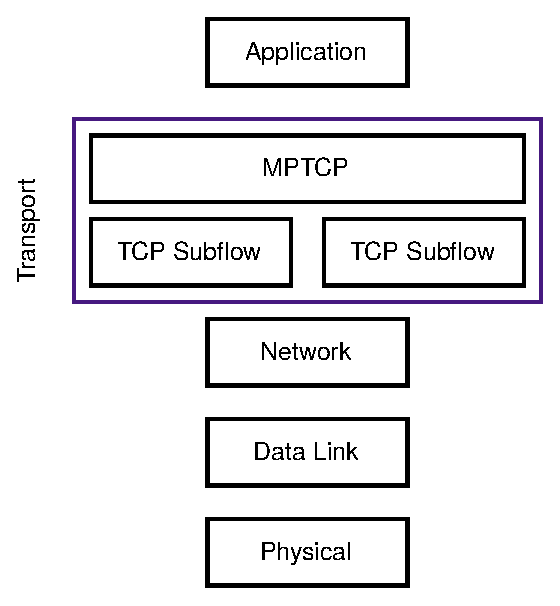
\includegraphics[width=.6\textwidth]{img/mptcp/mptcp_str}
    \caption{Transport Layer Structure.}
    \label{fig:TransportLayerStructure}
\end{figure}

\paragraph{} The \textbf{path management} is responsible for finding and using the available paths between two end hosts.
This part is also responsible for the advertisement of other alternative addresses to hosts and to set up new sub-flows.

\paragraph{} At the \textbf{packet scheduler} is where the byte stream received from the application is divided into
segments to transmit them on any one of the sub-flows available. Also in this part, the
connection-level re-ordering is performed whenever the packets are received from the TCP sub-flows.

\paragraph{} The \textbf{congestion control} part is responsible for coordinating between sub-flows to maintain the congestion control mechanism. This coordination is responsible for scheduling segments between sub-flows and the transfer rate as well.

\paragraph{} The \textbf{sub-flow interface} is in charge of transmitting on the specified path, the segments received from
the packet scheduler. On receipt of a segment, it passes the data to the packet scheduler for connection-level reassembly.

\paragraph{} Since MPTCP underneath uses TCP for network compatibility, it ensures reliable and in-order delivery.

\subsubsection{Connection Handling}
To establish a new connection, an application has to open a TCP socket, which will enable the initial TCP sub-flow. After the initial TCP connection, if both hosts support MPTCP capability, the MPTCP session can start on both hosts. The connection set up is explained, as shown in Fig.~\ref{fig:ConnectionHandling} \cite{barreia2014multipath}.
\paragraph{}To establish a new sub-flow from the Host A to Host B, the Host A receives from the DNS that it can connect Host B at the Address 1. Same three-way handshake mechanism is used similar for connection set up like normal TCP, but it carries MPTCP specific information which is only understood by the end system.

\paragraph{}The MP CAPABLE option is added on the handshake to allow either host to inform each other that they support MPTCP capability. The overall process is explained in Fig.~\ref{fig:ConnectionHandling}. The MPTCP session is now complete, from this point we explain how to add new sub-flows on an MPTCP session. At any point, either host can try to establish new sub-flows.

\begin{figure}[h]
    \centering
    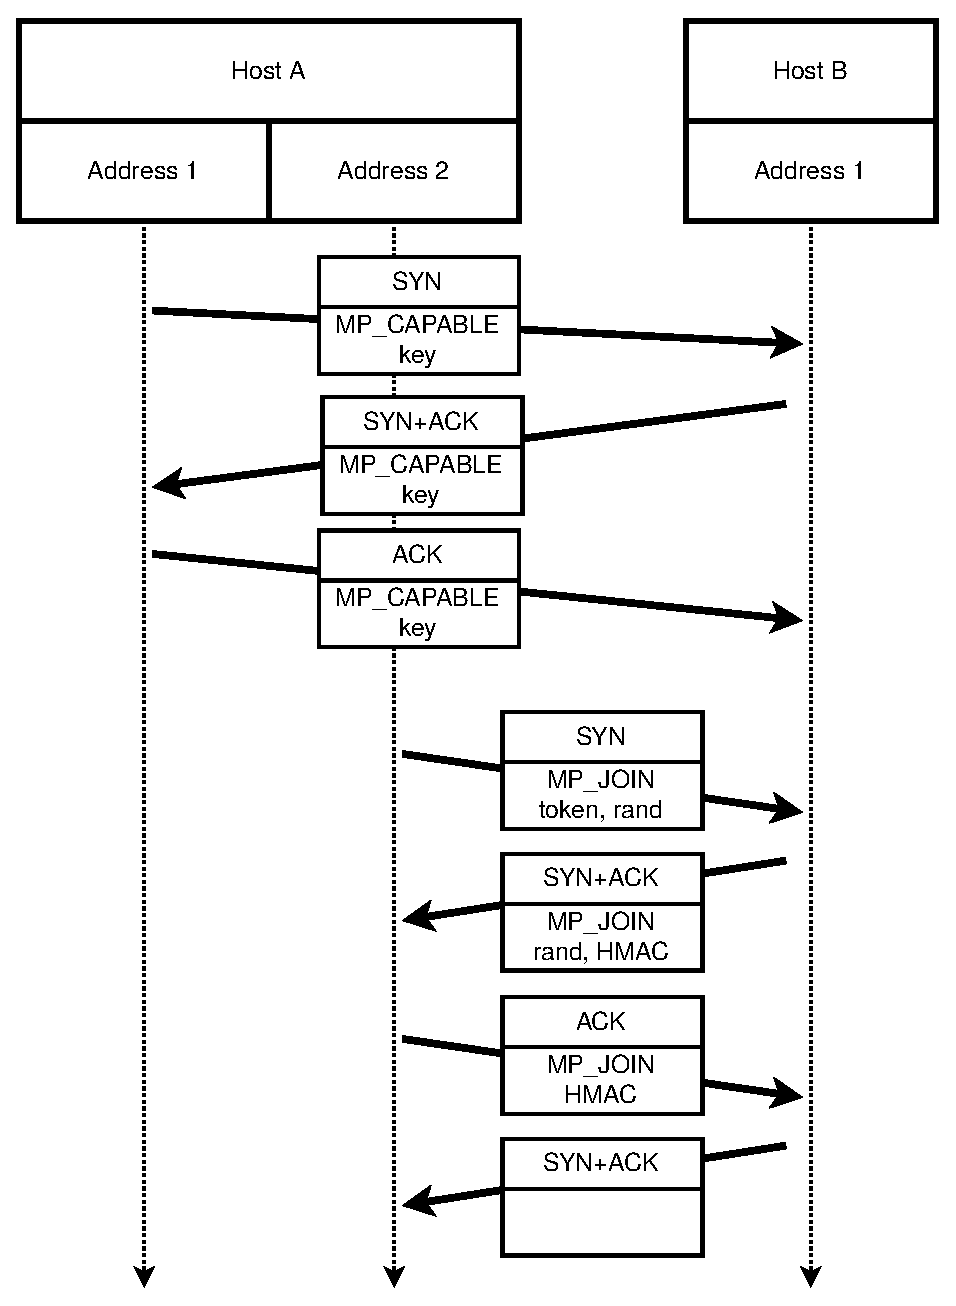
\includegraphics[width=.7\textwidth]{img/mptcp/mptcp_con}
    \caption{Transport Layer Structure.}
    \label{fig:ConnectionHandling}
\end{figure}

\paragraph{} Assume that Host A wants to create a sub-flow between its Address 2 and Host B Address 1. Again a
new TCP three-way handshake starts, but the option in use is different because now new sub-flows that will be created need to be attached to the existing MPTCP session. The option that will be used to build new sub-flows will be MP\_JOIN. Host A can establish new sub-flow using the addresses <A.2,B.1>, Host
An Address 2 with Host B Address 1, but it needs to be joined to the correct context in Host B. To achieve this, Host A attaches token B to the MP\_JOIN option. Host B responds with SYN and ACK, with MP JOIN option without a token, because Host A already has a state for that sub-flow. Then Host A sends ACK with the MP JOIN, in the context of Host B. And the final ACK is sent, and the sub-flow is ready to be used.

%MPTCP\cite{scharf2013multipath} is a recent drop in replacement for TCP. It is backward compatible, transparent to the application protocol. MPTCP supports mobility and multihoming. MPTCP utilize multiple network interface available to a device to speed up data transfer rate. MPTCP is just an extension of TCP\cite{mptcpsurvey}. It adds MPTCP layer on top of TCP and provides a congestion control algorithm. Normal TCP is a variation of MPTCP with a single sub flow. There are several challenges in designing the congestion control algorithm for MPTCP.
%%MPTCP is designed with these 
%
%\subsubsection{The Architectural Priciples}
%Application connects using regular socket API. MPTCP manages underlying TCP connections called sub-flow. Subflow is responsible for transferring data between hosts. MPTCP acts as a sub-layer in the stack shown in Fig.~\ref{fig:mptcpstack}. MPTCP uses additional signal using TCP optional header.
%
%\begin{figure}[h!]
%\centering
%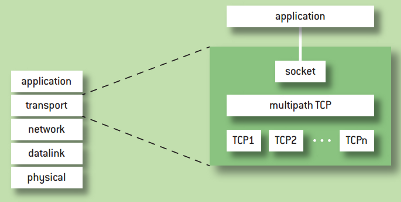
\includegraphics{img/mptcp/paasch1}
%\caption{MultiPath TCP in the TCP/IP Stack}
%\label{fig:mptcpstack}
%\end{figure}
%There are three phases in MPTCP:
%\begin{enumerate}
%    \item Connection Establishment
%    \item Add new sub-flow
%    \item Transmit data on the MPTCP connection.
%\end{enumerate}
%
%\textbf{Connection Establishment:}
%MPTCP establishes a connection using normal TCP's three-way handshaking. During connection establishment phase, MPTCP adds $MP_CAPABLE$ option with it the $SYN$ packet. If the server has MPTCP supported then it adds a $MP_CAPABLE$ option with the $SYN+ACK$ packet. And final $ACK$ packet also contain $MP_CAPABLE$ option. MPTCP (server or client) add a random key for security with its $SYN$ packet. 
%
%\begin{figure}[h!]
%\centering
%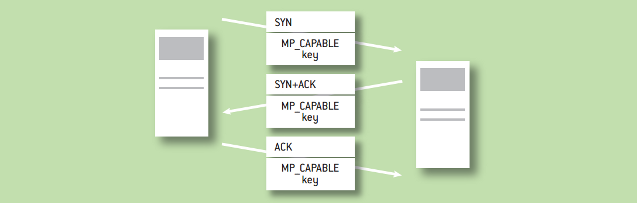
\includegraphics[width=\linewidth]{img/mptcp/paasch2}
%\caption{Three-way handshaking to establish MPTCP connection}
%\label{fig:ConnectionEstablishment}
%\end{figure}
%Three-way handshaking is shown in Fig.~\ref{fig:ConnectionEstablishment} create one MPTCP sub-flow to an interface. To use another path, MPTCP needs to add another sub-flow using a three-way handshake. However, this sub-flows need to be identified properly. Normal TCP identified by 4 tuple of $<src_ip,dst_ip,src_port,dst_port>$. MPTCP cannot use this as this tuple is host dependent. And network middlebox like NAT can change them. So MPTCP needs something more. 
%
%\begin{figure}[h!]
%    \centering
%    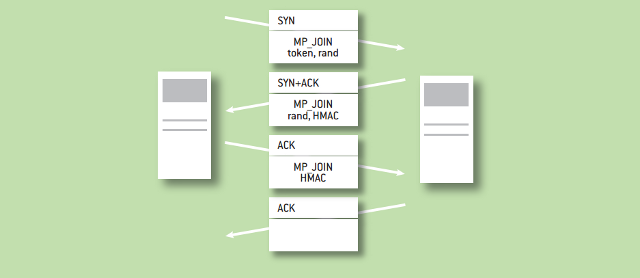
\includegraphics[width=\linewidth]{img/mptcp/paasch3}
%    \caption{}
%    \label{fig:4way}
%\end{figure}
%
%\textbf{Create additional sub-flow:} MPTCP uses 4 way handshaking shown in Fig.~\figurename{fig:4way} to add sub-flow. To add extra sub-flow, MPTCP uses the $MP_JOIN$ option with a $SYN$ packet. The $MP_JOIN$ option used to authenticate the sub-flow. Here $token$ is the truncated hash of key it receives during $MP_CAPABLE$ exchange. In this phase, two parties first exchange random nonce and then it compute HMAC based on the nonce and forward it to another party. Once both parties receive the $ACK$ for the random nonce it shared, the sub-flow is established.

\subsubsection{Data transfer and congestion control:}
As all the sub-flows are added, data can be transmitted between two hosts. MPTCP need a congestion control algorithm. A straightforward extension of TCP congestion control algorithm may be unfair to the single-path TCP.
Paas \textbf{et. al.} in \cite{PaaschMptcp} suggested a simple solution by using TCP independently for each path. However, their results show that MPTCP dominates in the bandwidth utilization.

\textbf{Link Increases Algorithm (LIA):} Using simple TCP in each path make single tcp strave. So Raiciu \textit{et. al.} proposes LIA to couple multiple path and use and aggresiveness factor to control the subflow window increament\cite{LIARFC6356}. The formulas without aggressive factor are as follows:
For each $ACK$, increase $w_r$ by 
$$min\left( \frac{max_{i\epsilon \mathcal{R}_u} w_i/rtt_i^2}{\left(\sum_{i\epsilon \mathcal{R}_u}w_i/rtt_i\right)^2}, \frac{1}{w_r}\right) $$
And one packet, decrease by $$\frac{w_r}{2}$$

where $\mathcal{R}_u$ path available to a user. $w_r$ congestion window size at path $r$.  $w_i$

\textbf{OLIA:} All sub-flows may not go through a distinct path. It may happen that 2 or more sub-flows are going through the same bottleneck. LIA will try balance between them. As paths are same, This two sub-flow start behaving like individual TCP flow. That will unfair to other normal TCP flow, as MPTCP will grab more share to the bottleneck. So LIA is not Pareto optimal\cite{OLIARamin2012}. Khalili \textbf{et. al.} propose a modification to the LIA algorithm name as \textit{Oportunistic Link Increases Algorithm} (OLIA).

On ack receive event, window will increase as per
\begin{equation}
\frac{w_r/rtt_r^2}{\left( \sum_{p\in\mathcal{R}_u}w_p/rtt_p\right)^2} + \frac{\alpha_r}{w_r}
\end{equation}

\begin{equation}
\alpha_r = \left\lbrace 
\begin{array}{ll}
\frac{1/|\mathcal{R}_u|}{|\mathcal{B}\smallsetminus \mathcal{M}|}  &\mbox{if} \hspace{0.3cm} r \in \mathcal{B}\smallsetminus\mathcal{M}\neq\emptyset   \\
- \frac{1/|\mathcal{R}_u|}{|\mathcal{M}|} \hspace{1cm}&\mbox{if} \hspace{0.3cm} r \in \mathcal{M} \hspace{0.3cm}\mbox{and}\hspace{0.3cm}\mathcal{B}\smallsetminus\mathcal{M}\neq \emptyset \\
0 & \mbox{otherwise}
\end{array} \right. 
\end{equation}


\textbf{Balanced Linked Adaptation (Balia):}
LIA and OLIA  suffer from the problem of on the unfair bandwidth allocation when it bottleneck with normal TCP flow. Walid \textit{et. al.} describe the balanced linked increases algorithm in \cite{walid2015balanced}. Balia balances trade off between TCP-Friendliness and algorithmic responsiveness.


%MPTCP uses coupled congestion control algorithm which is also known as LIA\cite{LIARFC6356}. However, LIA is not Pareto optimal\cite{OLIARamin2012}. It decreases the bandwidth utilization of other TCP flows on the Internet. So Khalili \textit{et. al.} suggested using OLIA, as new more conservative congestion control algorithm for MPTCP to avoid the more aggressive behavior. Ferlin \textit{et. al.} argued that it not the case when the path does not share any bottle neck\cite{MPTCP-SBD}. They developed a mechanism to detect shared bottleneck call MPTCP-SBD.
%Currently, available congestion algorithms are LIA, OLIA, BALIA and wVegas\cite{wVegas}. Apart from wVegas, all are an ack driven algorithm. Gonzalez \textit{et. al.} suggested a hybrid algorithm\cite{Balia-wvegas} using delay as well as the ack. \cite{aschedulermptcp,blestschedular,scheadulerformptcp} show several ways of scheduling a packet in a path over other. Hwang \textit{et. al.} suggested in \cite{scheadulerformptcp} that for small data transmission it is better to use single though single rather than using multipath as multipath need more time to setup. As flows can go through a heterogeneous path. It may cause Head-of-the line blocking. So \cite{blestschedular} suggested predictive scheduling algorithm BLEST reduce Head-of-the-Blocking. Other than congestion control algorithm and scheduling algorithm, research has been done in combined congestion control algorithm\cite{outofordermptcp}, performance tuning \cite{optimization}, multimedia streaming \cite{streaming}.


\subsection{Transmitting short-lived flows efficiently}

None of the above solutions have addressed the issue of short-lived connections. A large part of the traffic on the Internet in short-lived connection \cite{kheirkhah2015short}. A short-lived connection does not last enough to get out of slow start phase and transmit data in much lesser speed. It is a problem for the web server and middle boxes like router near to heavily loaded web server. It needs to retain connection and associated resources for the longer time. 

To address this issue Dukkipati \textit{et. al.} from Google suggested to increase initial congestion window size to least 10mss\cite{google-long-initcwnd} from 1mss. In general, it takes up to 3 round-trip time to reach congestion window to 10 MSS. For short flows like web browsing, Most of the time it does not have enough data to transmit after 4 RTT. TCP also take 1.5 RTT during connection establishment phase for three-way handshaking. In \cite{google-fast-open}, Radhakrishnan \textit{et. al.} from Google suggested that we can send during connection establishment phase, which saves time. However, this also not enough for short-lived connection over a long-fat link. Browser produces a very larger number of short-lived flows. Each of those connection goes through single TCP connection. Each of those connection needs to go through the similar issue. 

\subsection{SPDY}
As part of Google's "Let make the web faster" initiative, SPDY have been developed as an experimental protocol\cite{spdy}. SPDY offers a way to tries make the web faster from the application layer. The goals of SPDY are:
\begin{itemize}
    \item Overall reduction in 50\% of page load time.
    \item Easy deployability. SPDY uses TCP as the underlying transport protocol, so it does not require to change anything.
    \item It should not require any changes in web content. i.e. it should be transparent to both user and website developer.
\end{itemize}

\subsubsection{Design and features}
SPDY adds and extra session layer on top of normal SSL layer of HTTPS. It is shown in Fig.~\ref{fig:spdy.design}. SPDY does not change usual HTTP methods like GET or POST. However it add its own frame format for encoding and data transmission. 
\begin{figure}[h]
    \centering
    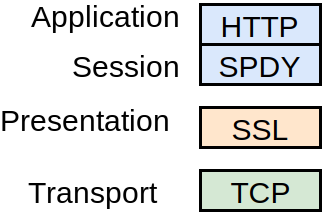
\includegraphics[width=\linewidth]{img/spdy/spdy_design}
    \caption{SPDY design}
    \label{fig:spdy.design}
\end{figure}

SPDY is a multiplexed stream base protocol. Its streams are bi-directional. SPDY aims to achieve low latency through basic and advanced features.
\textbf{Basic features}
\begin{itemize}
    \item \textbf{Multiplxed streams}: It will multiplex multiple streams over a single TCP connection between server and client. It uses concurrent transmission of streams.
    \item \textbf{Request Prioritization:} Client can request as many objects it wants from the server. But it may happen that one stream is clogging the connection. So, SPDY provides an option to give prioritization between streams so that it can block some stream at the time of congestion.
    \item \textbf{HTTP header compression:} SPDY compresses request header and response header resulting in a lesser number of byte in transmission.
\end{itemize}

\textbf{Advanced Feature}
\begin{itemize}
    \item \textbf{Server Push:} SPDY have an option to push objects to the client before it even asks for. It is useful in case of loading a page for the first. Standard an HTML page contain huge number object to enrich the browsing experience. In this case, the server knows what client is going to ask for, but the client may require time process the page then ask the content from the server. Push will help in enriching the experience by putting in the tip of client's finger.
    \item \textbf{Hint:} Server Push is useful. However, a client may not require all of the objects as it may be in their cache. So, SPDY provides a header filed to tell the client what are the object it supposed to ask and the server will be ready to serve those.
\end{itemize}


SPDY is a session layer. It maintains a persistent TCP connection called session between server and client. Then it send multiple streams in interleaved fashion Fig.~\ref{fig:http-timing-diagram}

\begin{figure}[h]
    \centering
    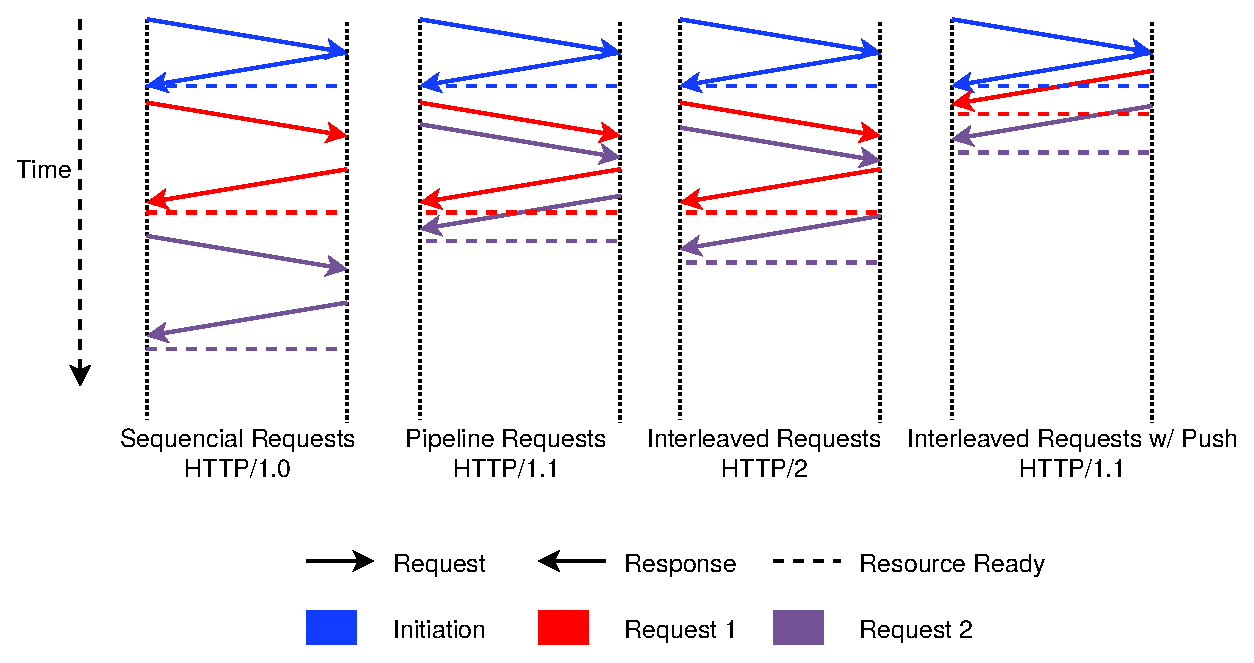
\includegraphics[width=0.7\linewidth]{img/spdy/http-timing-diagram}
    \caption{Comparison of time to fetch a HTTP request.}
    \label{fig:http-timing-diagram}
\end{figure}


%To solve this Google introduced experimental protocol SPDY\cite{spdy}. To avoid slow-start phase, Google multiplexed a large number of connection through a single TCP connection. SPDY become the standard from HTTP/2.0.
In \cite{howspeedis}, Wang \textit{et. al.} show that uses of SPDY performs better with short-lived connections. SPDY decreases the retransmission count. However, SPDY hurts under high packet loss as it uses single TCP connection and that TCP connection decreases its window size drastically. 

In \cite{canspdymake}, Eikhatib \textit{et. al.} shows that SPDY will work better only when a browser has to fetch large number small files from the server. Chinnaga \textit{et. al.} developed tool to test SPDY's perform\cite{scalabilitySPDY}. In \cite{han2015anatomy}, Han \textit{et. al.} explains how SPDY's performance can be improved using MPTCP.

Although SPDY is good, it suffers from the head-of-the-blocking. If one TCP packet gets lost in the network, TCP will not release rest of the packet, until it recovers the lost packet. As SPDY is stream multiplexing protocol, this scheme, all stream have to wait for the lost packet, which does not belong to them. Underlying protocol for SPDY is TCP. TCP does not support mobility. So, SPDY can not support mobility. To overcome these issues, Google developed Quick UDP Internet Connections(QUIC).

\subsection{QUIC}
Quick UDP Internet Connections (QUIC) is an experimental
protocol developed by Google. It is designed to provide
Security and reliability along with reduced transport latency. Google has already deployed QUIC protocol on their servers and has a client implementation in their web browser Chrome. We have shown a comparison with HTTP/2 in the layering approach in Fig.~\ref{fig:quic-protocolstack}. It is built on the top of UDP. Itself contain congestion control and loss recovery like TCP. The advantage of QUIC is that it provides encapsulate complete setup similar to TLS and HTTP combined.

\begin{figure}[h]
    \centering
    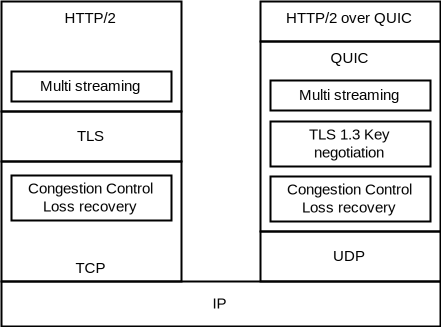
\includegraphics[width=0.7\linewidth]{img/quic/quic-protocolstack}
    \caption{QUIC protocol stack}
    \label{fig:quic-protocolstack}
\end{figure}

\begin{figure}[h]
    \centering
    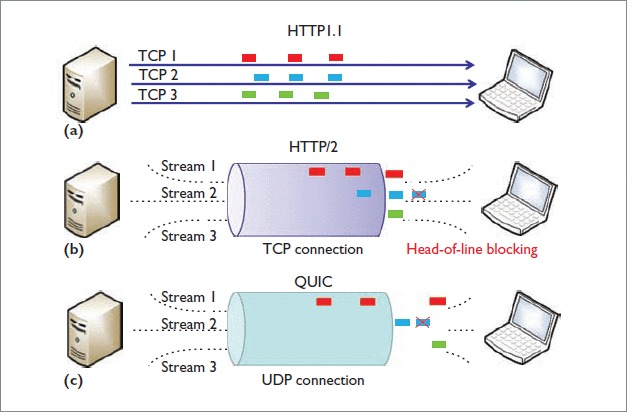
\includegraphics[width=.6\textwidth]{img/quic/transmission_compare}
    %    \includegraphics[width=.6\textwidth]{quick1}
    \caption{QUIC Multiplexing.}
    \label{fig:Quic1}
\end{figure}

\paragraph{} QUIC multiples several streams over the same QUIC UDP connection. Fig.~\ref{fig:Quic1} \cite{carlucci2015http} shows that with HTTP/1.1 a client can only use one resource at a time whereas with QUIC a client can send multiple HTTP requests and receive multiple responses over the same UDP socket. HTTP/1.1 web browsers attempt to minimize the impact of the head of the line blocking (HOL) by opening multiple concurrent HTTP connections, typically up to
six. The QUIC multiplexing feature has been inherited from
SPDY.

\begin{figure}[h]
    \centering
    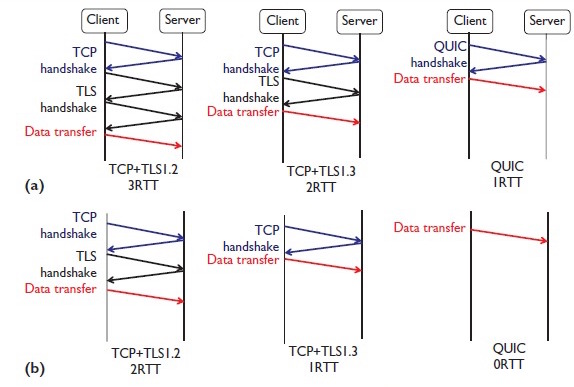
\includegraphics[width=.6\textwidth]{img/quic/quicrrtcompare}
    \caption{Connection establishment of different protocols.}
    \label{fig:Quic2}
\end{figure}

\paragraph{} One of the important features of QUIC is that it can connect to a client with 0-RTT if there was a connection between them previously. The can reduce the huge overhead of reconnection compared TCP dependent protocols. Fig.~\ref{fig:Quic2}\cite{quicisquic} clearly shows the way QUIC and other protocols differs based on their connection establishment procedure. 
%
%\begin{figure}
%    \centering
%    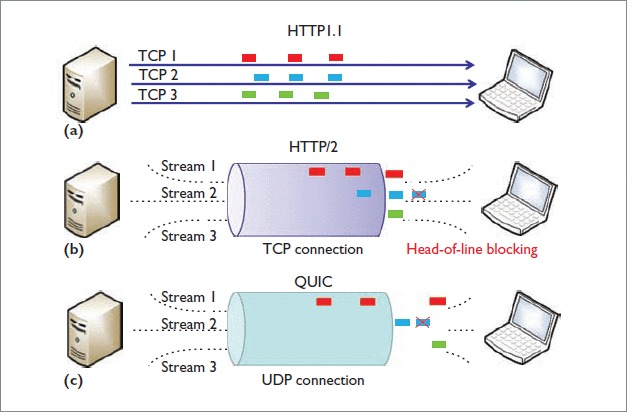
\includegraphics[width=.6\textwidth]{img/quic/transmission_compare}
%    \caption{Comparison of connection RTT.}
%    \label{fig:connectiontime}
%\end{figure}
%QUIC\cite{quic} is another experimental transport protocol developed by Google on top of UDP to make the web faster. Like SPDY it is also a stream multiplexing protocol, But it uses UDP as the underlying protocol. As UDP does not provide reliability or congestion control and flow control, it handles them by itself only. By providing congestion control by itself, it overcomes the problem of head-of-the-blocking. QUIC does not use any IP: Port as a connection identifier. It uses some unique identifier as a connection identifier. It helps QUIC in achieving Mobility.
%
%QUIC need 1 RTT time for connection establishment for the first time. After that, it can reuse the existing connection and archives 0RTT connection establishment. 

In \cite{quicmakewebfast}, Biswal \textit{et. al.} experimentally found that QUIC load pages quicker than HTTP/2 under poor network conditions. QUIC's performance also increases with increase in a size of objects and number of objects on a page.

Megyesi \textit{et. al.} presented a comparison study of QUIC, SPDY, and HTTP\cite{quicisquic}. They found that QUIC load page faster than HTTP. However, they also concluded that HTTP works better for larger object size.